\section{Introduction}
\label{sec:intro}

\begin{figure*}[t]
\centering
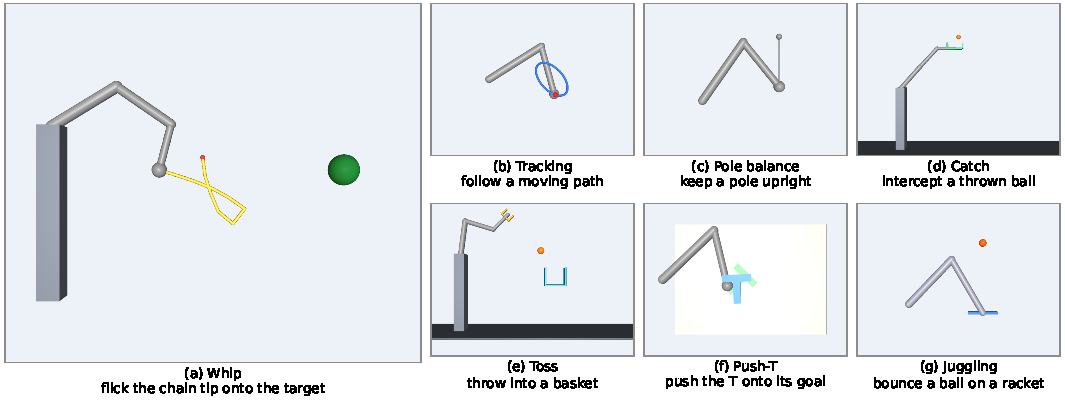
\includegraphics[width=\textwidth]{fig_tasks}
\caption{The seven tasks use planar MuJoCo arms (two links by default, three for whip). Each panel is a MuJoCo render under nominal parameters, taken from a classical teacher's rollout on a calibration seed. Whip (a), the main test bed, must flick a passive chain so that its tip hits the target. Script: \texttt{figures/make\_task\_renders.py}.}
\label{fig:tasks}
\end{figure*}

Claims that a learned controller beats a classical one steer which methods researchers pursue and which ones practitioners deploy, so the comparison behind such a claim has to hold up. It is often weaker than it looks, and our own first experiment shows how. A residual policy (a learned correction added to the classical controller's command), trained with proximal policy optimisation (PPO), beat the untuned computed-torque teacher on a 2-DoF tracking task by 16.7\% in root-mean-square tracking error (RMSE) without disturbances. After a two-parameter gain retune of the teacher, the advantage disappeared: the learned side was 7.1\% worse, with a 95\% confidence interval (CI) of $[-13.8, +0.3]\%$ (setting S1 in Table~\ref{tab:cross}). The gap was a tuning gap, not a learning gap.

This paper asks a narrower question than ``does learning win'': \emph{what extra ingredient does a learned student need to beat its classical teacher?} Candidate ingredients are more information (privileged state), better optimisation (reinforcement learning, RL, on top of the teacher), a richer model class (generative students), and more data. To answer under one set of rules, we built a benchmark with an explicit protocol and report every deviation from it. We study planar arms in one simulator on tracking, juggling and whip, a task in which the arm flings a chain so that its tip reaches a distant target. Whip is the only task with real \emph{headroom}, meaning room above the strongest classical pipeline: an oracle that knows the true plant parameters and the chain state scores far higher. All claims are scoped to this protocol and to this simulator.

Our answer is this. Under a fair, pre-specified and budget-disclosed protocol, no learning method beat the strongest classical baseline by +10\pp. On whip, the one task with headroom, a large share of the gain came from a decision rule, \emph{robust plan selection}: scoring candidate swings under several plausible plant parameters instead of trusting one estimate. The classical side can use the same rule, and on the second locked set the learned side keeps a lead of +5.6\pp\ [0.6, 10.6] that does not exclude 10\pp.

We make four contributions, K1--K4. Their evidence differs. K1 rests on the protocol's own audit, an access log of test evaluations and a git-order check of the rules. K2 rests on the seed sets listed per setting in Table~\ref{tab:settings}. Only whip (S7) uses once-only \emph{locked} test sets (TEST-B, TEST-C, TEST-D); the other settings use the reused test set TEST ($n{=}50$), the reused holdout set HOLD, or fresh seeds. K3 rests on the locked sets TEST-C and TEST-D, and K4 on fresh but unlocked seeds.
\begin{enumerate}
\item[\textbf{K1}] \textbf{An audited protocol} (Section~\ref{sec:protocol}): classical tooling extended on the same footing as the learner's, budgets reported on three axes with over-runs disclosed, rules pre-specified in time-stamped, version-controlled written records (\emph{hypothesis cards}), a \emph{sanity gate} (a check that a learner can learn a deliberately injected, known-learnable correction before its failure on the real task is interpreted), and the access log. The gate passed only marginally (+10.2\pp\ against a +10\pp\ threshold). Its first lesson was that a default exploration scale left PPO unable to learn a learnable correction.
\item[\textbf{K2}] \textbf{A cross-setting result with one whip qualification} (Section~\ref{sec:k2}): in 8 tracking, juggling and whip settings no learned method beat the strongest classical baseline by the +10\pp\ bar. On whip, a learned estimator is ahead of the upgraded classical one by +5.6\pp\ [0.6, 10.6] when both use robust plan selection. An advantage of 10\pp\ or more cannot be excluded.
\item[\textbf{K3}] \textbf{A headroom decomposition on realistic whip} (Section~\ref{sec:k3}): a ladder in which each step (rung) gives the classical pipeline one more piece of privileged information. On TEST-C, true parameters add +17.6\pp\ [12.6, 22.6] over fitted ones. On the second locked set TEST-D (gap +18.0\pp), robust plan selection alone recovers 0.59 [0.36, 0.82] of the gap with a classical Laplace ensemble (C-ens: parameter samples drawn from a Gaussian approximation around the fitted parameters) and 0.90 [0.68, 1.16] with learned estimators.
\item[\textbf{K4}] \textbf{A multimodal-teacher result} (Section~\ref{sec:k4}): a multimodal teacher gives several different plans for the same situation. Replacing it by a canonical teacher that gives one consistent plan raised every student's success by 17.5--33.5\pp, while the best generative student added only +5.0\pp\ [$-0.3$, 10.2] over an MLP.
\end{enumerate}

Two sources of fragility run through these results, and we state them here rather than in the limitations. First, in 3 of the 8 settings the RL learner did not learn, so those settings cannot show that classical is better. Second, the classical comparator on whip, C-ens, was added after the learned method had already beaten the original classical baseline; the final contrast is pre-specified, but the comparator was built with the learned result in view.

The gap we address is that comparisons of classical and learned control rarely combine four things. These are a classical side tuned and extended as far as the learner, a manipulator whose simulated physics is independent of the controllers' own model, rules fixed and audited before testing, and a decomposition of where the remaining headroom lies. To our knowledge no prior work combines all four (the literature search ended in October 2026; Section~\ref{sec:related}). We fill it with an extended classical ladder, the audited protocol, and a headroom ladder on whip. Section~\ref{sec:protocol} describes the protocol, Section~\ref{sec:setup} the setup, and Section~\ref{sec:results} the results for K2--K4; Sections~\ref{sec:discussion} and~\ref{sec:limitations} interpret them and state their limits. Every number in the text is traced to a result file, a README line or a code constant (\texttt{numbers\_check.md} in the accompanying repository); the appendices give the deviations, budgets and the remaining experiments.
